\documentclass{article}
\usepackage[T1]{fontenc}
\usepackage[french]{babel}
\usepackage{graphicx} % Required for inserting images
\usepackage{amsmath}
\usepackage{geometry}
\usepackage{indentfirst} % Ajoute l'indentation au premier paragraphe de chaque section
\usepackage{amssymb}
\usepackage{hyperref}
\usepackage{biblatex}


\bibliography{Biblio}

\title{Calcul Quantique Adiabatique }
\author{Côme Périn \\ Sam Gubernator}
\date{Décembre 2023}
\geometry{margin=3cm}


\begin{document}

\begin{figure}[h]
    \centering
    
\includegraphics[scale=0.35]{rsc/Logo_ENSEIRB-MATMECA-Bordeaux_INP.png}
    \label{fig:enter-label}
    \maketitle
\end{figure}


\tableofcontents
\newpage


\section{Introduction}

Le calcul quantique défini le fait d'utiliser les propriétés quantiques de la matière afin de résoudre des problèmes : factorisation de nombres, recherche de période, etc. Une approche répandue du calcul quantique consiste à modifier l'état d'un système quantique à travers une succession de porte logique quantiques (porte de Hadamard, de Pauli \dots). Cette approche \emph{basée sur le circuit} implique une modification "instantanée" du système quantique.

\medskip

\noindent Le calcul adiabatique se soustrait à l'usage de porte quantique et fait évoluer le système de façon continue, en utilisant la notion de \emph{Hamiltonien}.
Contrairement au calcul basé sur le circuit, elle annonce plusieurs avantages dont la diminution des erreurs et l'optimisation des problèmes complexes.

\medskip

\noindent Cette méthode de calcul est fondée sur l'application du \emph{Théorème adiabatique}.

\section{Système quantique}

Afin d'expliquer le principe du calcul quantique adiabatique, il est nécessaire de voir quelques bases de physique quantique.

\medskip

\noindent On travaille sur un \emph{système quantique} (constitué de particules quantiques par exemple). L'état du système quantique est modélisée en tout point et à tout instant par une fonction d'onde $\Psi(x,t)$. Les densités de probabilité du système sont données par $|\Psi(t)|^2$.

\medskip

\noindent L'évolution de cette fonction d'onde est régie par l'équation de Schrödinger.

\subsection{Équation de Schrödinger}

Établie en 1925 par Erwin Schrödinger, cette équation permet de décrire l'état d'un système quantique à tout instant. Elle peut s'écrire de la façon suivante : 

\begin{equation}
    \label{schro}
    i\hbar\frac{d|\Psi(t) \rangle}{dt} = \hat{H}|\Psi(t)\rangle
\end{equation}

\noindent $\hbar=\frac{h}{2\pi}$ où $h$ est la constante de Planck. \\
\noindent Le terme $\hat{H}$ est appelé opérateur hamiltonien. \cite{wikipedia2023schrodinger}

\medskip

Quelques mots sur cet opérateur sont nécessaires à la compréhension de la suite\dots

\subsection{Hamiltonien}

D'un point de vue purement mathématique, un hamiltonien $A$ est représenté par une matrice hermitienne, \emph{i.e.} qui vérifie : 
$$(A^T)^* = A$$

Cependant, d'un point de vue physique :

\medskip

\noindent Dans le contexte de l'équation de Schrödinger, \textit{le hamiltonien, dépendant du temps en général, est l'observable correspondant habituellement à l'énergie totale du système.} (\href{https://fr.wikipedia.org/wiki/%C3%89quation_de_Schr%C3%B6dinger}{Wikipedia})

\medskip

\noindent Le hamiltonien sert donc à décrire l'état global de l'environnement du système à chaque instant et son évolution est un point clé pour la suite du processus. \cite{wiki2023hamiltonian}

\subsection{Évolution du système}

L'évolution continue de l'état du système est modélisée par $H(t)$. Lors d'une expérience (quantique potentiellement), l'état du système va évoluer entre $t_0$ et $t_f$. Ainsi, $\tau = t_f - t_0$ est donc la durée d'évolution du système. La valeur de $\tau$ est très importante dans le processus de calcul quantique adiabatique.

\section{Théorème adiabatique}

\subsection{États propres}

Il est possible de démontrer que les solutions de l'équation de Schrödinger~(\ref{schro}) s'écrivent comme le produit d'une fonction $|\Psi(t)\rangle$ et d'autres fonctions dont il ne sera pas nécessaire de connaître l'expression ici.

\medskip

\noindent Dans la suite, la solution de l'équation et $|\Psi(t)\rangle$ ne seront pas distingués pour un souci de simplicité.

\medskip

$|\Psi(t)\rangle$ est un état propre, ce qui signifie qu'il satisfait :  

$$\forall t>0, H(t)|\Psi(t)\rangle=E(t)|\Psi(t)\rangle$$

Où $E(t)$ décrit l'évolution d'un niveau d'énergie du système au cours du temps.

\medskip

\noindent Donc $E(t)$ est une valeur propre de $H$ pour l'état propre $|\Psi(t)\rangle$. De plus, il apparait que la notion d'état propre propose une généralisation physique du vecteur propre mathématique.

\medskip

\noindent Il existe une multitude de fonctions d'ondes de ce type, associées à autant de niveaux d'énergies. Ainsi, l'indiçage suivant est possible :

$$\forall t>0, H(t)|\Psi_n(t)\rangle=E_n(t)|\Psi_n(t)\rangle$$

\noindent Les niveaux d'énergie $E_n(t)$ sont non-dégénérés. \\ Cela signifie que pour un $E_i(t)$ il existe un unique état propre $|\Psi_i(t)\rangle$ vérifiant la relation précédente.

\begin{figure}[h]
    \centering
    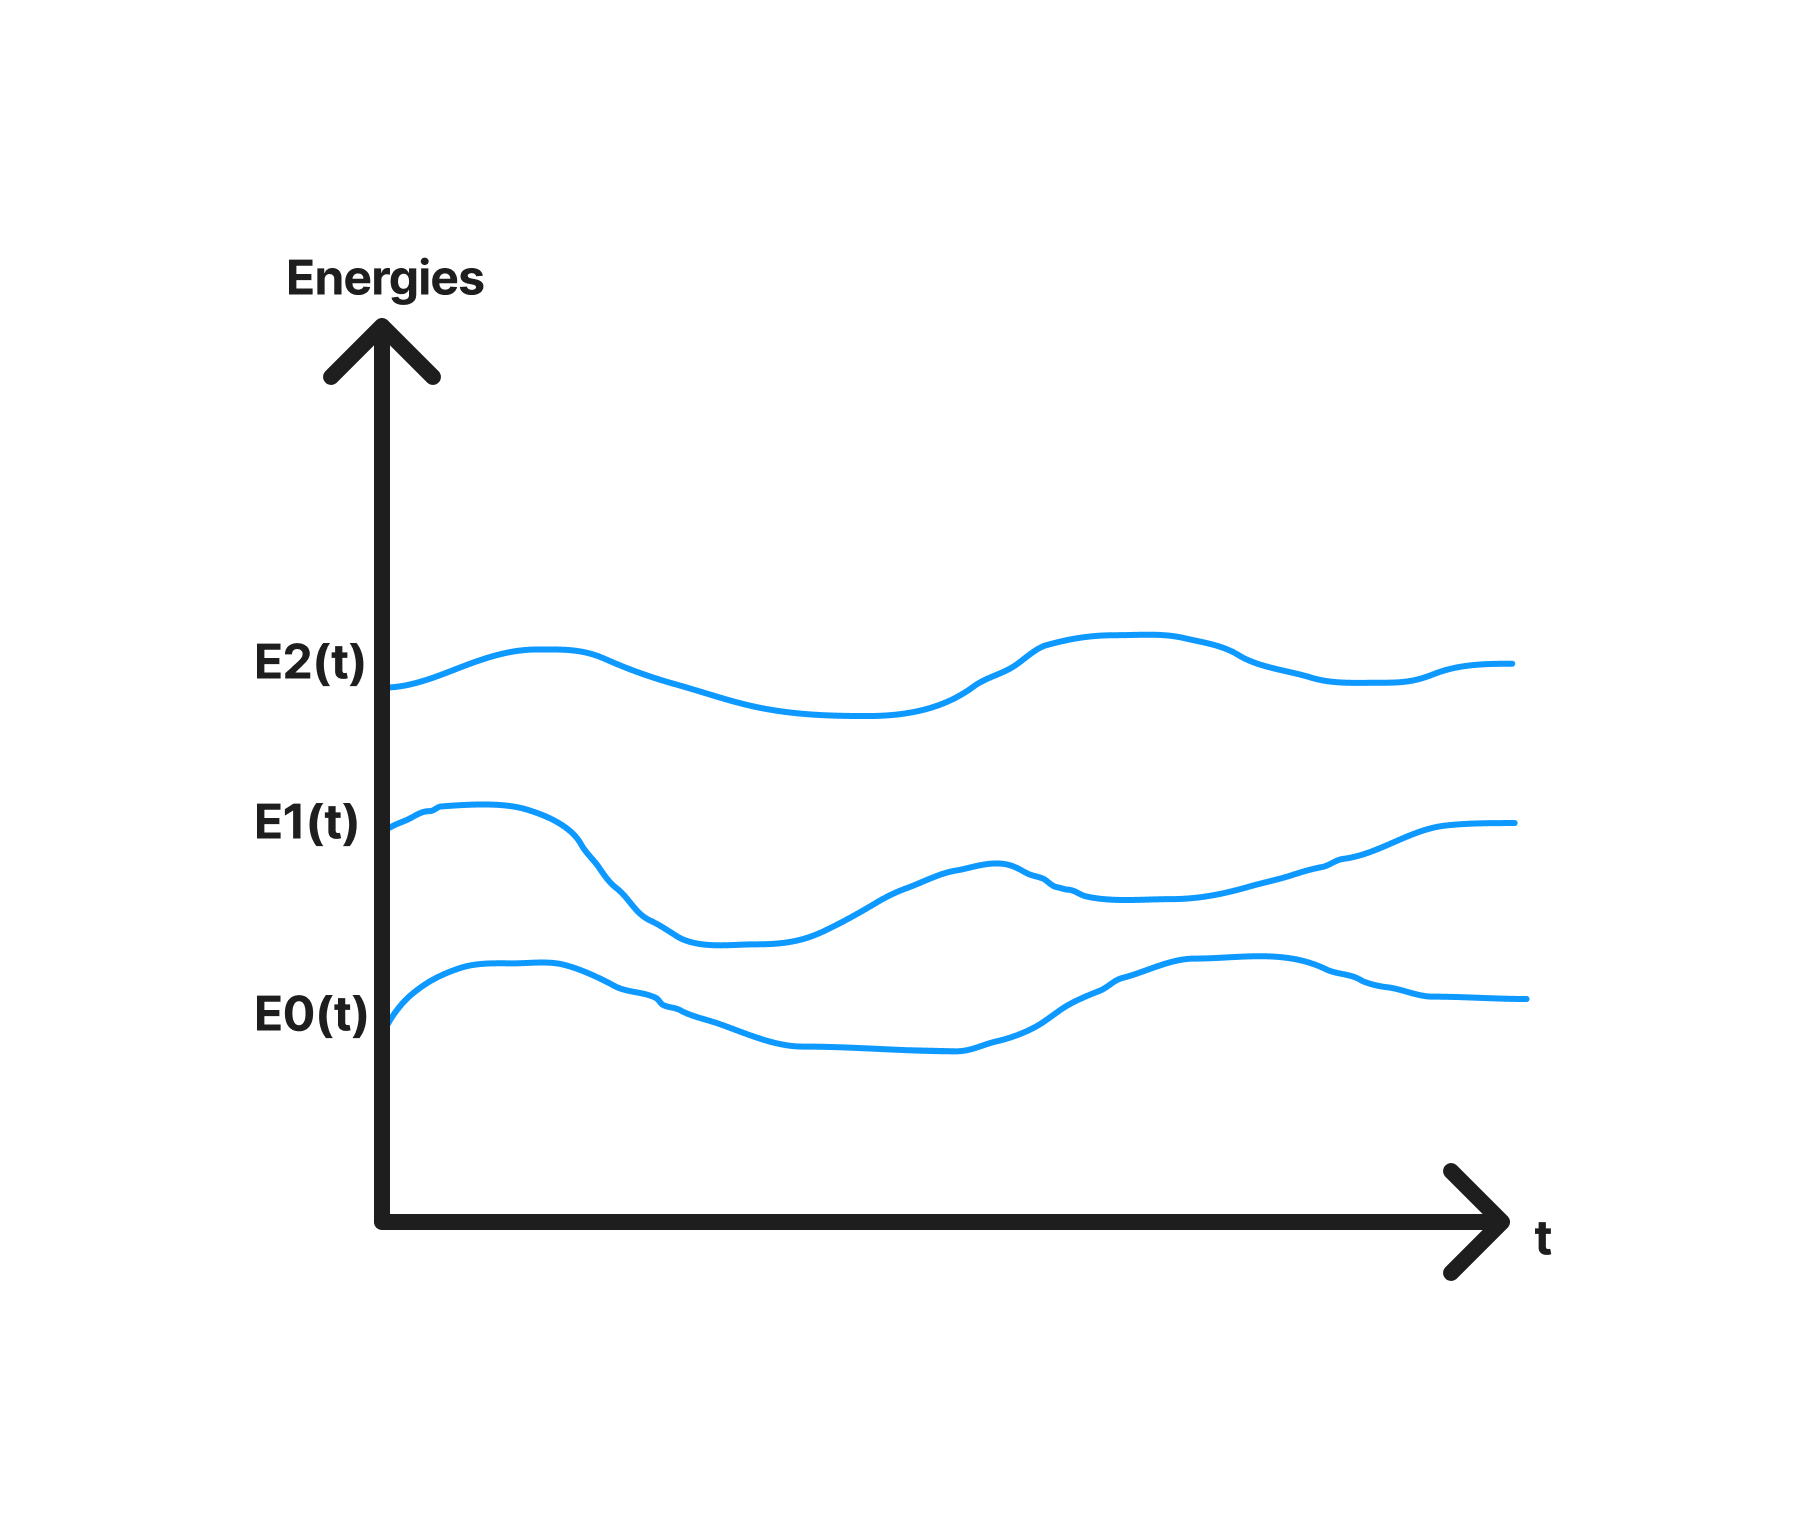
\includegraphics[scale=0.25]{rsc/energies.png}
    \caption{Illustration arbitraire de l'évolution des niveaux d'énergie au cours du temps}
    \label{fig:enter-label}
\end{figure}

\newpage
\subsection{Énonciation}

Munis dès lors des outils explicités précédemment, il est possible d'énoncer le \emph{théorème adiabatique} sur lequel se base le calcul quantique adiabatique.

\medskip

Soit un système quantique décrit par $\Psi(t)$. Initialement, le système possède une énergie $E_i(t_0)$. Par ce qui précède, on déduit que $\Psi(t_0)=\Psi_i(t_0)$. 

\bigskip

Si : 

\begin{itemize}
    \item $\forall t\in [t_0,t_f] \text{  } E_{i-1}(t)<E_i<E_{i+1}$ (énergies suffisamment éloignées)
    \item $\tau \xrightarrow{} \infty$ (évolution suffisamment lente)
\end{itemize}

\bigskip

Alors $\forall t\in[t_0, t_f], \Psi(t)=\Psi_i(t)$ et $E(t)=E_i(t)$. En particulier, $\Psi(t_f)=\Psi_i(t_f)$ et $E(t_f)=E_i(t_f)$.

\medskip

\noindent Ce processus est décrit comme étant \emph{adiabatique}. Il permet au système de modifier progressivement sa forme fonctionnelle afin de rester en phase avec l'évolution du niveau énergétique initial.

\medskip

\noindent Il est donc possible d'effectuer une transformation sur un système quantique tout en suivant l'évolution de l'énergie initiale : on ne "bascule" pas dans d'autres niveaux d'énergies. \cite{wiki2023adiabatictheorem} \cite{mitocw2023}

\section{Calcul adiabatique quantique}

Il est possible de trouver une solution optimale pour un problème complexe en partant d'une solution optimale pour un problème plus simple, que l'on a fait évoluer de façon continue vers un problème complexe. Le calcul ne requiert aucune porte quantique puisqu'il repose sur l'évolution continue du système (là où une porte quantique modifie le système instantanément). La lecture de la solution se fait en mesurant l'état final.

\medskip

\noindent L'idée est de trouver un hamiltonien complexe $H_f$ dont l'état fondamental répond au problème posé. Initialement, on part d'un hamiltonien plus simple et le système est placé dans l'état fondamental correspondant. L'enjeu est ensuite de faire évoluer $H_0$ vers $H_f$ sans jamais quitter l'état fondamental. Une fois l'opération réussite, une mesure dans l'état final permet de répondre au problème complexe de manière optimale. \cite{wiki2023adiabaticquantumcomputing} \cite{delahaye2016memoire}

\medskip
\noindent Le principal avantage de cette méthode est la certitude de répondre au problème de manière optimale (à condition que l'adiabaticité soit respectée). En effet, le niveau d'énergie fondamental traduit la solution la plus stable (et donc la meilleure).

\subsection{Exemple d'application}

Le calcul adiabatique quantique est une méthode efficace pour traiter des problèmes complexes, comme le problème du voyageur de commerce. Ce dernier consiste à déterminer le chemin le plus court permettant de visiter chaque ville une fois, tout en revenant à la ville de départ. Pour ce faire, on utilise un hamiltonien, qui, dans son état fondamental, modélise les liaisons possibles entre les villes. Trois types d'opérateurs sont utilisés dans ce hamiltonien : un pour représenter les liens entre les villes, un autre pour les villes elles-mêmes, et un dernier pour identifier les villes visitées. En encodant le chemin dans le hamiltonien et en appliquant cette méthode, il est possible de trouver une solution en temps polynomial, ce qui est nettement plus rapide que les méthodes classiques. \cite{arxiv2018quantum}


\newpage
\section{Caractéristiques de la méthode}

Cette méthode serait équivalente aux opérations unitaires effectuées sur des qubits à travers des portes en termes de performances. Elle a pour but d'empêcher un système quantique de changer d'état, et supprimerait les phénomènes de dissipation quantique, pouvant entraîner de la décohérence.\medskip

\noindent En effet, le but étant de rester dans l'état fondamental, les perturbations extérieures ne pourront pas faire "descendre" le système vers un niveau d'énergie inférieur. Mieux, si l'extérieur a tendance à faire diminuer le niveau d'énergie du système, il lui sera plus difficile de changer d'état. 

\bigskip

\noindent Seulement, cette méthode soulève une question quant au temps nécessaire à l'obtention de résultats, afin de déterminer si celle-ci est bien plus rapide qu'un calcul classique. En théorie, la vitesse d'exécution dépend de la différence d'énergie entre l'état initial et l'état visé. Plus cette différence est grande, plus il est possible d'accélérer le calcul et donc plus cette méthode est efficace en comparaison à un équivalent classique.

\printbibliography

\end{document}